\begin{notationpage}

\vskip 15mm

First recall the conventional multiindex notation. Let $\NN_0$ denote the nonnegative integers. A multiindex $\alpha = (\alpha_1, \alpha_2, \ldots, \alpha_n) \in \NN_0^n$ is an $n$-tuple of nonnegative integers. The degree of a multiindex is $|\alpha| = \alpha_1 + \alpha_2 + \cdots + \alpha_n$. Multivariate exponentiation is defined as follows. For $x = (x_1, x_2, \ldots, x_n) \in \RR^n$,
\[
  x^\alpha = x_1^{\alpha_1}x_2^{\alpha_2} \cdots x_n^{\alpha_n}.
\]
Here we will use the convention $0^0 = 1$ so that for example $(x, y, z)^{(0, 1, 0)} = y$. We will use $e_i \in \RR^n$ to represent the canonical unit vector
\[
  e_i = (0, \ldots, 0, 1, 0, \ldots, 0)
\]
which can also be interpreted as a multiindex so for example
\[
  (x,y,z)^{2e_1 + e_3} = x^2z
\]

The multinomial formula gives a convenient expansion for multinomial powers. Let $k \in \NN_0$. Then
\[
  {(b_1 + b_2 + \cdots + b_n)}^k = \sum_{|\alpha| = k} \binom{k}{\alpha} b^\alpha
\] 
where the multinomial coefficients are defined
\[
  \binom{k}{\alpha} = \frac{k!}{\alpha_1! \alpha_2! \cdots \alpha_n!}.
\]
Note that the multinomial expansion sums over all multiindeces $\alpha \in \NN_0^n$ of degree $k$.

We denote the standard euclidean inner product
\[
  \langle x,y \rangle = x_1y_1 + x_2y_2 + \cdots + x_n y_n
\]
where $y = (y_1, y_2, \ldots, y_n) \in \RR^n$ and the Euclidean norm 
\[
  \|x\| = \sqrt{x_1^2 + x_2^2 + \cdots + x_n^2}
\]
We may slightly abuse notation by using the inner product and norm in different dimensions, even in the same equation. This can be excused if one views each euclidean space $\RR^n$ as embedded in the sequence space $\ell^2(\RR^\NN)$ in which the inner product and norm are equivalent.

When discussing hyperplanes in $\RR^n$ we index them by a unit normal vector, $\omega \in S^{n-1}$, and distance from origin $-\infty < p < \infty$, and we write for example the implicit hyperplane equation $\langle x, \omega \rangle = p$. Note that $\langle x, -\omega \rangle = -p$ represents the same hyperplane. It is perhaps more correct, in later defining the Radon and Gaussian Radon transforms, to identify these indexes and define the transforms over a projective space. We omit this discussion as it is not relevant within the scope of this work.
\begin{figure}[h]
  \centering
  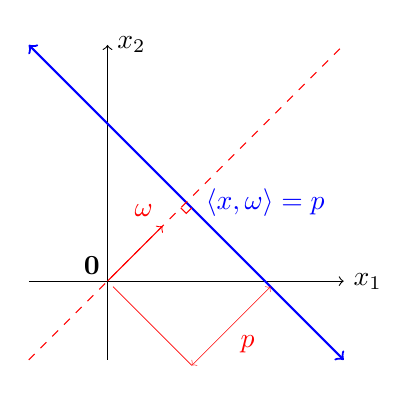
\begin{tikzpicture}[plane/.style={<->,thick,blue},
        vector/.style={->,red},
        axis/.style={->,black}]
    %draw axes
    \draw[axis] (-1,0) -- (3,0) node[anchor=west]{$x_1$};
    \node at (-.2,.2) {$\mathbf{0}$};
    \draw[axis] (0,-1) -- (0,3) node[anchor=west]{$x_2$};
    %draw plane
    \draw[plane] (-1, 3) -- (3, -1) node[midway, right]{~$\langle x, \omega\rangle = p$};
    %draw projection angle and orthogonal vector
    \draw[red,dashed] (-1,-1) -- (3,3);
    \def\ra{.07};
    \draw[red] (1-\ra, 1-\ra) -- (1,1-2*\ra) -- (1+\ra,1-\ra);
    \draw[vector] (0,0) -- (0.7,0.7) node[above left]{$\omega$};
    %draw extension line
    \draw[very thin, red] (\ra, -\ra) -- (1+\ra, -1-\ra);
    \draw[<->,very thin, red] (1+\ra, -1-\ra) -- (2+\ra, -\ra) node[midway,below right]{$p$};
  \end{tikzpicture}
  \caption{Hyperplane equation}\label{fig:HypEq}
\end{figure}

Unless otherwise indicated all measures are Euclidean measures, that is the Borel measure assocciated with the standard Euclidean metric on a given space. In particular the Euclidean measure on a hyperplane of $\RR^n$ is equivalent to the Euclidean measure on $\RR^{n-1}$. We chose for convenience to denote measures by their associated variable such as $dx$, $dp$, $dz$, and others. It should be stated that this notation, while uniform, is context dependent. For example in the integrals
\[
  \int_{\RR^n}~dx \qquad \text{and} \qquad \int_{\langle x, \omega\rangle = p} ~dx,
\]
the measure $dx$ is to be understood as the $n$-dimensional and $(n-1)$-dimensional Euclidean measure respectively.

% \begin{enumerate}[A) ]

%   \item \bf{Spaces}       
%         \begin{itemize}
%           \item $\ccL^2(\IR^d)$, all square integrable functions.
%           \item $\ccD(\IR^d)$, all cadlag functions.
%           \item $\ccC(\IR^d,\IR)$, all continuous functions from $\IR^d$ to $\IR$.
%           \item $\ccC_0(\IR^d,\IR)$, those functions in $\ccC(\IR^d,\IR)$ that vanish at infinity.
%           \item $\ccC_{00}(\IR^d,\IR)$, those functions in $\ccC(\IR^d,\IR)$ that have compact support.        
%         \end{itemize}
%         \vskip 1mm          

%   \item \bf{General Operators}       
%         \begin{itemize}
%           \item $\cL$, $\cM$, $\hat\cL$, $\hat\cM$ : generators of a semigroup
%           \item $\cP_t$, $\cQ_t$, $\hat\cP_t$, $\hat\cQ_t$ : the corresponding semigroups                    
%         \end{itemize}
%         \vskip 1mm          

%   \item \bf{Specific Operators}   
%         \begin{itemize}
%           \item $Lf(x) = \nabla \cdot A(x) \nabla ~ f (x)$
%           \item $\tilde Lf(x) = \nabla \cdot \tilde A(x) \nabla ~ f (x)$
%           \item $L^h f(x) = \frac{1}{h^2} ~ \sum\limits_{z \in \ZZ^d} (f(x+hz)-f(x)) ~ \Cxhz$
%           \item $\tilde L^h f(x) = \frac{1}{h^2} ~ \sum\limits_{z \in \ZZ^d} (f(x+hz)-f(x)) ~ \tCxhz$
%           \item Semigroups: $P_t = e^{tL}$, $\tilde P_t = e^{t\tilde L}$, 
%                 $P_t^h = e^{tL^h}$, $\tilde P_t^h = e^{t\tilde L^h}$
%         \end{itemize}
%         \vskip 1mm          

%   \item \bf{Markov Processes}
%         \begin{itemize}
%           \item $X_t^{(h)}$ is the process on $h\ZZ^d$ with generator $L^h$. 
%           \item $\tilde X_t^{(h)}$ is the process on $h\ZZ^d$ with generator $\tilde L^h$. 
%           \item $X_t$ is the process on $\IR^d$ with generator $L$. 
%           \item $\tilde X_t$ is the process on $\IR^d$ with generator $\tilde L$. 
%         \end{itemize}

%   \mynewpage{1}

%   \item \bf{Dirichlet Forms} \\
%         In general, $\ccE_\cM(f,g) = - \langle \cM f | g \rangle$. In $\ccL^2 (\IR^d,\mu)$, the
%         inner product is defined as
%         \begin{equation*}
%           \langle  f | g \rangle = \int\limits_{\IR^d} f(x) g(x) dx
%         \end{equation*}
%         while in $\ccL^2 (h\ZZ^d,\mu^h)$ it is defined as
%         \begin{equation*}
%           \langle  f | g \rangle = h^d ~ \sum\limits_{x \in h\ZZ^d} f(x) g(x)  .                           
%         \end{equation*}
%         Note the rescaling factor $h^d$. Therefore, the various Dirichlet forms are
%         \begin{itemize}
%           \item $\ccE(f,g) = - \displaystyle\int [\nabla \cdot A \nabla ~ f](x) ~ g(x) ~ dx$
%           \item $\tilde \ccE(f,g) = - \displaystyle\int [\nabla \cdot \tilde A \nabla ~ f](x) ~ g(x) ~ dx$
%           \item $\ccE^h(f,g) = \frac{1}{2} ~ h^{d-2}                 
%                                   ~\sum\limits_{x,z \in \ZZ^d} (f(x+hz)-f(x))~(g(x+hz)-g(x)) ~\Cxhz$               
%           \item $\tilde \ccE^{h,\varepsilon} (f,g) = \frac{1}{2} ~ h^{d-2} ~ \sum\limits_{x,z \in \ZZ^d} 
%                                         (f(x+hz)-f(x)) ~ (g(x+hz)-g(x)) ~ \tCxhz$                      
%         \end{itemize}
%         \vskip 1mm          

%   \item \bf{Our Standard Mollifier} \\
%         For each $\varepsilon > 0$, we define a standard mollifier:
%         \begin{equation*}
%             \eta_\varepsilon (y) = \frac{1}{\varepsilon^d} \eta \left( \frac{y}{\varepsilon} \right)
%         \end{equation*}
%         where $\eta$ is defined as follows:
%         \begin{equation*}
%             \eta(y) =
%             \begin{cases}
%               c_d \exp \left( \frac{1}{\|y\|^2 -1} \right) & \hbox{ if } \|y\| < 1 \cr
%               0                     & \hbox{ otherwise }
%             \end{cases}
%         \end{equation*}
%         with $c_d$ chosen such that $\| \eta \|_1 = 1$.
%         \vskip 1mm          

%   \item \bf{Miscellaneous}   
%         \begin{itemize}
%           \item $c$ is a positive constant for which the actual value does not matter and
%                     can change from line to line. Sometimes an index will be added for clarity.
                    
%         \end{itemize}

% \end{enumerate}

\end{notationpage}
